\documentclass[12pt]{article}
\usepackage{latexsym,amssymb,amsmath} % for \Box, \mathbb, split, etc.
% \usepackage[]{showkeys} % shows label names
\usepackage{cite} % sorts citation numbers appropriately
\usepackage{path}
\usepackage{url}
\usepackage{verbatim}
\usepackage[pdftex]{graphicx}

% horizontal margins: 1.0 + 6.5 + 1.0 = 8.5
\setlength{\oddsidemargin}{0.0in}
\setlength{\textwidth}{6.5in}
% vertical margins: 1.0 + 9.0 + 1.0 = 11.0
\setlength{\topmargin}{0.0in}
\setlength{\headheight}{12pt}
\setlength{\headsep}{13pt}
\setlength{\textheight}{625pt}
\setlength{\footskip}{24pt}

\renewcommand{\textfraction}{0.10}
\renewcommand{\topfraction}{0.85}
\renewcommand{\bottomfraction}{0.85}
\renewcommand{\floatpagefraction}{0.90}

\usepackage{accents}
\newcommand{\ubar}[1]{\underaccent{\bar}{#1}}
\makeatletter
\setlength{\arraycolsep}{2\p@} % make spaces around "=" in eqnarray smaller
\makeatother
\usepackage{stackengine}
% change equation, table, figure numbers to be counted inside a section:
\numberwithin{equation}{section}
\numberwithin{table}{section}
\numberwithin{figure}{section}

% begin of personal macros
\newcommand{\half}{{\textstyle \frac{1}{2}}}
\newcommand{\eps}{\varepsilon}
\newcommand{\myth}{\vartheta}
\newcommand{\myphi}{\varphi}

\newcommand{\IN}{\mathbb{N}}
\newcommand{\IZ}{\mathbb{Z}}
\newcommand{\IQ}{\mathbb{Q}}
\newcommand{\IR}{\mathbb{R}}
\newcommand{\IC}{\mathbb{C}}
\newcommand{\Real}[1]{\mathrm{Re}\left({#1}\right)}
\newcommand{\Imag}[1]{\mathrm{Im}\left({#1}\right)}
\DeclareRobustCommand{\brkbinom}{\genfrac[]{0pt}{}}
\newcommand{\norm}[2]{\|{#1}\|_{{}_{#2}}}
\newcommand{\abs}[1]{\left|{#1}\right|}
\newcommand{\ip}[2]{\left\langle {#1}, {#2} \right\rangle}
\newcommand{\der}[2]{\frac{\partial {#1}}{\partial {#2}}}
\newcommand{\dder}[2]{\frac{\partial^2 {#1}}{\partial {#2}^2}}
\usepackage{enumitem}
\newcommand{\nn}{\mathbf{n}}
\newcommand{\xx}{\mathbf{x}}
\newcommand{\uu}{\mathbf{u}}
\usepackage{tikz}
\usetikzlibrary{arrows}
\usetikzlibrary{positioning}
\usepackage{titlesec}
\newcommand{\junk}[1]{{}}
\usepackage{sectsty}
\usepackage{xcolor}
\newcommand*{\bfrac}[2]{\genfrac{}{}{0pt}{}{#1}{#2}}
\newcommand\myatop[2]{\left[{{#1}\atop#2}\right]} % "wrapper macro"

\makeatletter
\renewcommand*\env@matrix[1][\arraystretch]{%
	\edef\arraystretch{#1}%
	\hskip -\arraycolsep
	\let\@ifnextchar\new@ifnextchar
	\array{*\c@MaxMatrixCols c}}
\makeatother

\makeatletter
\renewcommand*\env@matrix[1][*\c@MaxMatrixCols c]{%
	\hskip -\arraycolsep
	\let\@ifnextchar\new@ifnextchar
	\array{#1}}
\makeatother

\definecolor{darkblue}{rgb}{0,0,0.4}
\usepackage[colorlinks = true,
linkcolor = darkblue,
urlcolor  = darkblue,
citecolor = darkblue,
anchorcolor = darkblue]{hyperref}
% set two lengths for the includegraphics commands used to import the plots:
\newlength{\fwtwo} \setlength{\fwtwo}{0.45\textwidth}
% end of personal macros

\begin{document}
\DeclareGraphicsExtensions{.jpg}

\begin{center}
\textsc{\Large Statistical Pattern Recognition} \\[2pt]
	\textsc{\large Assignment 2}\\
	\vspace{0.5cm}
  Ali Gholami \\[6pt]
  Department of Computer Engineering \& Information Technology\\
  Amirkabir University of Technology  \\[6pt]
  \def\UrlFont{\em}
  \url{http://ceit.aut.ac.ir/~aligholamee}\\
    \href{mailto:aligholamee@aut.ac.ir}{\textit{aligholamee@aut.ac.ir}}
\end{center}

\begin{abstract}
In this assignment, we'll be focusing on the \textit{Bayes Classifier}. We'll work with \textit{Bayesian Discriminators} and \textit{Bayes Error}. The \textit{Bhattacharyya} error bound is also analyzed as an upper bound for the \textit{Bayes Classifier} error. The detailed computations of \textit{Bayesian Discriminators} are also given in an exact definition. Finally, we'll be going through a more practical example of a linear discriminator by classifying the flowers in the \textit{Iris} dataset.
\end{abstract}

\subparagraph{Keywords.} \textit{Linear Discriminator, Quadratic Discriminator, Bayes Classification, Bayes Error, Optimal Classification, Bhattacharyya Distance, Bhattacharyya Upper Bound, Iris Dataset, Iris Classification.}

\section{Quadratic \& Linear Discriminant Analysis}
We consider a classification problem in dimension $d=2$, with $k=3$ classes where:\\
$$
p(x\ |\ w_{i}) \sim N(\mu_{i}, \Sigma_{i}),\ \  i = 1, 2, 3
$$
and
$$
	\mu_1 = 	\renewcommand\arraystretch{1}
	\setlength\arraycolsep{6pt}
	\begin{bmatrix}
	0\\
	2\\
	\end{bmatrix},\ 
	\mu_2	 = 	\renewcommand\arraystretch{1}
	\setlength\arraycolsep{6pt}
	\begin{bmatrix}
	3\\
	1\\
	\end{bmatrix},\ 	
	\mu_3	 = 	\renewcommand\arraystretch{1}
	\setlength\arraycolsep{6pt}
	\begin{bmatrix}
	1\\
	0\\
	\end{bmatrix},
	\Sigma_{i}	 = \Sigma =	\renewcommand\arraystretch{1}
	\setlength\arraycolsep{6pt}
	\begin{bmatrix}
	1 & 0\\
	0 & \frac{1}{3}\\
	\end{bmatrix},
$$
\begin{enumerate}[label=(\alph*)]
	\item Calculate the discriminant function $g_{i}(x)$ for each class.
	
	\item Express your discriminant functions in the form of linear discriminant functions.
	
	\item Determine and plot the decision boundaries.
\end{enumerate}
\subsection*{Solution}
(a) The general form of a Bayesian discriminator is given below.
\begin{equation}\label{eq:1.1}
g_{i}(\underaccent{\bar}{x}) = 	-\frac{1}{2}(\underaccent{\bar}{x} - \underaccent{\bar}{\mu}_{i})^{T}\Sigma_{i}^{-1}(\underaccent{\bar}{x} - \underaccent{\bar}{\mu}_{i}) - \frac{1}{2}\log|\Sigma_{i}| + \log P(\omega_{i})
\end{equation}
In the problem case, the classes have the same covariance matrix, but the features have different variances.
Since the $\Sigma_{i}$ is diagonal, we'll have
$$
g_{i}(\underaccent{\bar}{x}) = 	-\frac{1}{2}(\underaccent{\bar}{x} - \underaccent{\bar}{\mu}_{i})^{T}
	\begin{bmatrix}
\sigma_1^{-2} & 0 & 0 & \dots & 0\\
0 & \sigma_2^{-2} & 0 & \dots & 0\\
0 & 0 & \sigma_3^{-2} & \dots & 0\\ 
\vdots & \vdots & \vdots & \ddots & 0\\
0 & 0 & 0 & 0 & \sigma_N^{-2}\\
\end{bmatrix}
(\underaccent{\bar}{x} - \underaccent{\bar}{\mu}_{i}) - \frac{1}{2}\log \begin{vmatrix}
\sigma_1^{-2} & 0 & 0 & \dots & 0\\
0 & \sigma_2^{-2} & 0 & \dots & 0\\
0 & 0 & \sigma_3^{-2} & \dots & 0\\ 
\vdots & \vdots & \vdots & \ddots & 0\\
0 & 0 & 0 & 0 & \sigma_N^{-2}\\
\end{vmatrix} + \log(P(\omega_{i}))
$$
Since we have the following criteria:
$$
	(\underaccent{\bar}{x} - \underaccent{\bar}{\mu}_{i})^{T} = \begin{bmatrix}
	x[1] - \mu_{i}[1]\\
	x[2] - \mu_{i}[2]\\
	x[3] - \mu_{i}[3]\\
	x[4] - \mu_{i}[4]\\
	\vdots\\
	x[N] - \mu_{i}[N]\\
	\end{bmatrix}
$$
where $\mu_{iN}$ denotes the \textit{N}'th feature of class \textit{i}. Removing the constant term for different classes, which is $ x[k]^2$, we'll have the following results after the matrix multiplication and determinant computation:
\begin{equation}
	g_{i}(\underaccent{\bar}{x}) = -\frac{1}{2}\sum_{k=1}^{N}\frac{2x[k]\mu_{i}[k] + \mu_{i}[k]^2}{\sigma_k^2} - \frac{1}{2}\log\prod_{k=1}^{N}\sigma_k^2 + \log(P(\omega_i))
\end{equation}

One can simply find each discriminator, $g_{i}(\underaccent{\bar}{x})$, by replacing the given information in the problem description in the formula given above. Thus we'll have the following results for the section (a).
$$
	g_{1}(\underaccent{\bar}{x}) = -\frac{1}{2}(\frac{2x[1]*0 + 2}{1} + \frac{2x[2]*2 + 4}{\frac{1}{9}}) - \frac{1}{2}\log(1*\frac{1}{9}) + ?
$$
$$
g_{2}(\underaccent{\bar}{x}) = -\frac{1}{2}(\frac{2x[1]*3 + 3}{1} + \frac{2x[2]*1 + 1}{\frac{1}{9}}) - \frac{1}{2}\log(1*\frac{1}{9}) + ?
$$
$$
g_{3}(\underaccent{\bar}{x}) = -\frac{1}{2}(\frac{2x[1]*1 + 1}{1} + \frac{2x[2]*0 + 0}{\frac{1}{9}}) - \frac{1}{2}\log(1*\frac{1}{9}) + ?
$$
The simplified results are
$$
	g_{1}(\underaccent{\bar}{x}) = -18x[2] - \frac{1}{2}\log\frac{1}{9} - 19
$$
$$
	g_{2}(\underaccent{\bar}{x}) = -3x[1] + 9x[2] - \frac{1}{2}\log\frac{1}{9} - 6
$$
$$
	g_{3}(\underaccent{\bar}{x}) = -x[1] - \frac{1}{2}\log\frac{1}{9} - \frac{1}{2}
$$
\noindent\rule{\textwidth}{.5pt}
(b) The final results given above where in the format of a linear discriminant already. In order to lighten everything up, just assume the linear discriminant function as:
$$
	g_{i}(\underaccent{\bar}{x}) = W_{2}x[2] + W_{1}x[1] + W_0
$$
where the value of $W_i$ is different for each of the discriminators.
$$
	g_{1}(\underaccent{\bar}{x}) \ \ \ W_2 = -18 \ \ W_1 = 0 \ \ W_0 =  - \frac{1}{2}\log\frac{1}{9} - 19
$$
$$
g_{2}(\underaccent{\bar}{x}) \ \ \ W_2 = 9 \ \ W_1 = -3 \ \ W_0 =  - \frac{1}{2}\log\frac{1}{9} - 6
$$
$$
g_{1}(\underaccent{\bar}{x}) \ \ \ W_2 = 0 \ \ W_1 = -1 \ \ W_0 =  - \frac{1}{2}\log\frac{1}{9} - \frac{1}{2}
$$
Each of the $g_{i}(\underaccent{\bar}{x})$ represent a discriminator plane in the \textit{3D} space.

\noindent\rule{\textwidth}{.5pt}
(c) Here are the plots of distributions and discriminators below. These are coded in Python using \textit{PyLab}.
\begin{figure}[!h]\centering
	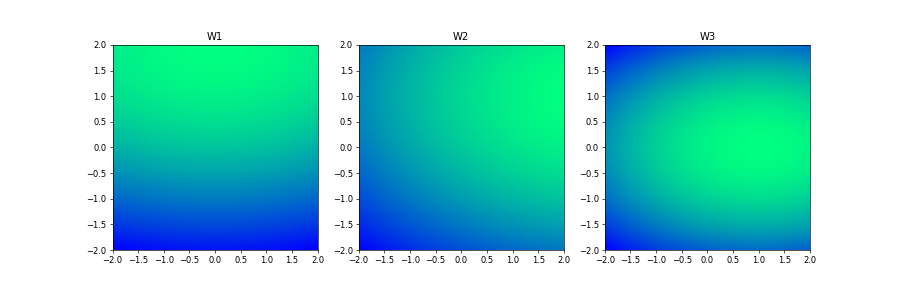
\includegraphics[width=0.8\textwidth]{1_c_1.png}
	\caption{Distributions of three classes described in the problem description.}
	\label{pl1}
\end{figure}
\begin{figure}[!h]\centering
	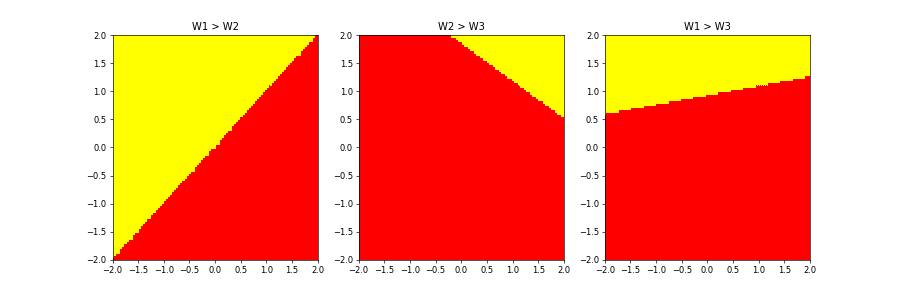
\includegraphics[width=0.8\textwidth]{1_c_2.png}
	\caption{Linear discriminators of Figure 1.1 distributions.}
	\label{pl2}
\end{figure}

\section{Bayes Decision Rule \& Bayes Error Boundaries}
Consider the following 2-class classification problem involving a single feature $x$. Assume equal class priors and $0-1$ loss function.
$$
p(x\ |\ w_1) = \begin{cases} 
2x &  0 \leq x \leq 1\\
0       &  otherwise
\end{cases} \ \ \ \ p(x\ |\ w_2) = \begin{cases} 
2-2x &  0 \leq x \leq 1\\
0       &  otherwise
\end{cases}
$$	
\begin{enumerate}[label=(\alph*)]
	\item Sketch the two densities.
	
	\item State the Bayes decision rule and show the decision boundary.
	
	\item What is the Bayes classification error?
	
	\item How will the decision boundary change if the prior for class w1 is increased to 0.7? 
\end{enumerate}
\section*{Solution}
(a) Figure 2.1, illustrates the density functions of these two classes. I've used the \textit{Seaborn} library to generate these density functions.
\begin{figure}[!h]\centering
	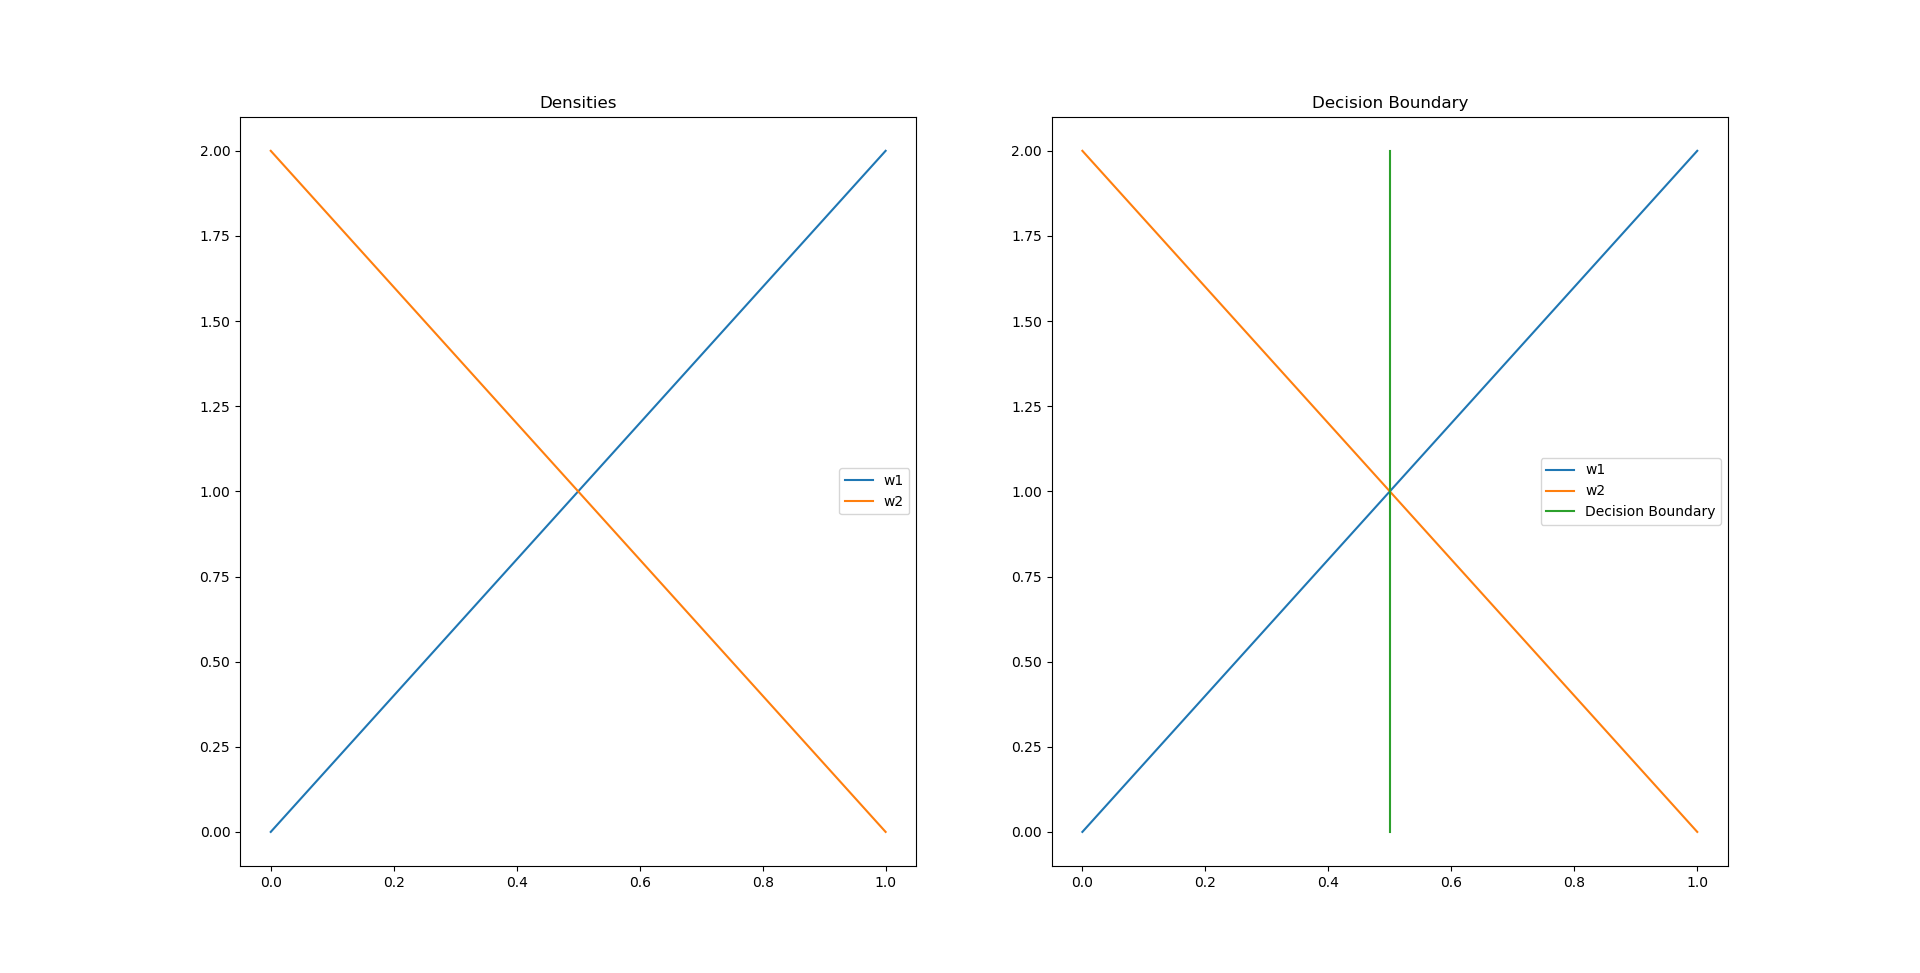
\includegraphics[width=0.7\textwidth]{2_1_1.png}
	\caption{Illustration of density functions of $w_1$(Blue) and $w_2$(Orange).}
	\label{density}
\end{figure}

\noindent\rule{\textwidth}{.5pt}
(b) We drive the Bayes decision rule for these two classes below. $g_1(x)$ and $g_2(x)$ represent the decision function for the classes 1 and 2 respectively.

$$
	g_i(x)\ \bfrac{\overset{\omega_i}{>}}{\overset{\omega_j}{<}}\ g_j(x)
$$
which is our decision baseline for the Bayes classifier. Since $g_i(x) = p(\omega_1\ |\ x)$, expanding the equation according to the Bayes rule and we get:
$$
	g_i(x) = \frac{p(\underaccent{\bar}{x}\ |\ \omega_i)P(\omega_i)}{p(\underaccent{\bar}{x})}
$$
Replacing the $g_i(x)$ in the decision baseline and we'll have the following results.
$$
	\frac{p(\underaccent{\bar}{x}\ |\ \omega_i)P(\omega_i)}{p(\underaccent{\bar}{x})}\  \bfrac{\overset{\omega_i}{>}}{\overset{\omega_j}{<}}\ \frac{p(\underaccent{\bar}{x}\ |\ \omega_j)P(\omega_j)}{p(\underaccent{\bar}{x})}
$$
Omitting the constant parts from both sides and replacing the equations from the problem description will result in the following decision function.
\begin{equation}
	g(x) = 4x - 2\ \bfrac{\overset{\omega_i}{>}}{\overset{\omega_j}{<}}\ 0
\end{equation}
Thus, the linear discriminant function can be displayed as so:
$$
	g(x) = 4x - 2
$$
in which the point $x = \frac{1}{2}$ is the separation point of two classes. The values greater than $\frac{1}{2}$ are assigned a label from class $i$. The values less the $\frac{1}{2}$ are assigned a label of class $j$.

\noindent\rule{\textwidth}{.5pt}
(c) Here is the Bayes classification error given in (2.2).
\begin{equation}
	\eps = \eps_1P(\omega_1) + \eps_2P(\omega_2)
\end{equation}
in which the $\eps_1$ and $\eps_2$ represent the probability of class 1 error by integrating the class 1 density over the region of class 2 and the probability of class 2 error by integrating the class 2 density over the region of class 1 respectively.
$$
	\eps_1 = \int_{R_2} p(\underaccent{\bar}{x}\ |\ \omega_1)d\underaccent{\bar}{x}
$$
$$
	\eps_2 = \int_{R_1} p(\underaccent{\bar}{x}\ |\ \omega_2)d\underaccent{\bar}{x}
$$
According the section (b), the discriminating point is $x = 0.5$. Correspondingly, the regions $R_1$ and $R_2$ can be easily driven like so:
$$
	R_1 = [0\ 0.5] \ \ \ \ R_2 = [0.5\ 1]
$$
By integrating the given equation (2.2) over the boundaries of these two regions, we'll have the following:
$$
	\eps_1 = \int_{0}^{0.5}(2x) dx = \frac{1}{4}
$$
$$
	\eps_2 = \int_{0.5}^{1} (2-2x)dx = \frac{1}{4}
$$
The final value for the Bayes error will be:
$$
	\eps = \frac{1}{4} * \frac{1}{2} + \frac{1}{4} * \frac{1}{2} = \frac{1}{4}
$$

\noindent\rule{\textwidth}{.5pt}
(d) Changing the prior probabilities for classes $\omega_1$ and $\omega_2$, the bias will be changed. We'll have the following biases as the prior probabilities.
$$
	P(\omega_1) = 0.7
$$
$$
	P(\omega_2) = 0.3
$$
Rewriting the likelihood ratio for these two classes, we'll have the following results:
$$
	\frac{p(\underaccent{\bar}{x}\ |\ \omega_1)}{p(\underaccent{\bar}{x}\ |\ \omega_2)}\  \bfrac{\overset{\omega_1}{>}}{\overset{\omega_2}{<}}\ \frac{P(\omega_2)}{P(\omega_1)}
$$
$$
	\frac{2x}{2-2x}\  \bfrac{\overset{\omega_1}{>}}{\overset{\omega_2}{<}}\ \frac{3}{7}
$$
which changes the final discriminant function, $g(x)$ to
$$
	g'(x) = 10x - 3\ \bfrac{\overset{\omega_1}{>}}{\overset{\omega_2}{<}}\ 0
$$

\section{Bayes Decision Boundary \& Bhattacharyya Error Bound}
Consider a two-category classification problem in two dimensions with
$$
p(x\ |\ w_{1}) \sim N(0, I),\ \ \ p(x\ |\ w_{2}) \sim N(\begin{bmatrix}
1\\
1\\
\end{bmatrix}, I)
$$
and
$$
P(\omega_1) = P(\omega_2) = \frac{1}{2}
$$
\begin{enumerate}[label=(\alph*)]
	\item Calculate the Bayes Decision Boundary.
	
	\item Calculate the Bhattacharyya error bound.
	
	\item Repeat the above for the same probabilities, but
	$$
	p(x\ |\ w_{1}) \sim N(0, \begin{bmatrix}
	2 & 0.5\\
	0.5 & 2\\
	\end{bmatrix}),\ \ \ p(x\ |\ w_{2}) \sim N(\begin{bmatrix}
	1\\
	1\\
	\end{bmatrix}, \begin{bmatrix}
	5 & 4\\
	4 & 5\\
	\end{bmatrix})
	$$
\end{enumerate}
\subsection*{Solution}
(a) The genera for of a Bayesian discriminator was discussed in (1.1). Comparing this to the linear classifier which can be displayed as below:
$$
	g_i(\underaccent{\bar}{x}) = W_{i1}^T\underaccent{\bar}{x} + W_{i0}
$$
where the weights are also given below:\\
$$
	W_{i1} = \frac{\mu_i}{\sigma^2}
$$
$$
	W_{i0} = \frac{-1}{2\sigma^2}\mu_{i}^T\mu_{i} + \log P(\omega_i)
$$
Since $\Sigma_i = \sigma^2I$ with $\sigma^2 = 1$(according to problem description) with equal prior probabilities($P(\omega_1) = P(\omega_2) = \frac{1}{2}$, the discriminator can be derived using the \textit{Euclidean Distance} of $x$ and $\mu$.
$$
	g_i(\underaccent{\bar}{x}) = (\underaccent{\bar}{x} - \underaccent{\bar}{\mu}_i)^T (\underaccent{\bar}{x} - \underaccent{\bar}{\mu}_i)
$$
we can simply find the $g_1(\underaccent{\bar}{x})$ and $g_2(\underaccent{\bar}{x})$ by replacing the parameters in the problem description. We'll get:
$$
	g_1(\underaccent{\bar}{x}) = (\underaccent{\bar}{x} - 0)^T(\underaccent{\bar}{x} - 0) = (\underaccent{\bar}{x})^2
$$	
$$
	g_2(\underaccent{\bar}{x}) = (\underaccent{\bar}{x} - \begin{bmatrix}
	1\\
	1\\
	\end{bmatrix})^T(\underaccent{\bar}{x} - \begin{bmatrix}
	1\\
	1\\
	\end{bmatrix}) = (\underaccent{\bar}{x} - 1)^2
$$	
In order to find the decision boundary, we'll coincide the two discriminators:
$$
	\underaccent{\bar}{x} = \frac{1}{2}
$$
Meaning that the decision boundary is the plane $\underaccent{\bar}{x} = \frac{1}{2}$.

\noindent\rule{\textwidth}{.5pt}
(b) The \textit{Bhattacharyya} error bound is an specific condition of \textit{Chernoff} error bound. This condition happens when $s = \frac{1}{2}$ in the \textit{Chernoff} bound formula. The \textit{Bhattacharyya} formula is given below.
\begin{equation}
	\eps_{n-B} = \sqrt{P(\omega_1) P(\omega_2)} \int \sqrt{p(\underaccent{\bar}{x}\ |\ \omega_1)p(\underaccent{\bar}{x}\ |\ \omega_2)}d\underaccent{\bar}{x} = e^{-\mu(s = \frac{1}{2})}
\end{equation}
If we have access to the parameters of two distributions we can derive the \textit{Bhattacharyya} error bound by computing the $\mu(s = \frac{1}{2})$ and replacing the result in the $e^{-\mu(s = \frac{1}{2})}$.
$$
	\mu(\frac{1}{2}) = \frac{1}{8}(\underaccent{\bar}{m}_2 - \underaccent{\bar}{m}_1)^T(\frac{\Sigma_1 + \Sigma_2}{2})^{-1}(\underaccent{\bar}{m}_2 - \underaccent{\bar}{m}_1) + \frac{1}{2}\ln \frac{|\frac{\Sigma_1 + \Sigma_2}{2}|}{\sqrt{|\Sigma_1| |\Sigma_2|}}
$$
after some minor matrix multiplication, we'll get the following results:
$$
	\mu(\frac{1}{2}) = (\frac{1}{8})(4) = \frac{1}{2}
$$
The \textit{Bhattacharyya} error bound will be $\eps_{n-B} = e^{-\frac{1}{2}}$.

\noindent\rule{\textwidth}{.5pt}
(c) $g_1(\underaccent{\bar}{x})$ and $g_2(\underaccent{\bar}{x})$ can be easily computed using the \textit{general form} of the Bayes classifier.
$$
	g_1(\underaccent{\bar}{x}) = -\frac{1}{2}(\underaccent{\bar}{x} - 0)^T\renewcommand\arraystretch{1}
	\setlength\arraycolsep{6pt}\begin{bmatrix}
	\frac{8}{15} & \frac{2}{15}\\
	\frac{2}{15} & \frac{8}{15}\\
	\end{bmatrix}(\underaccent{\bar}{x} - 0) - \frac{1}{2}\log \frac{15}{4} + \log \frac{1}{2}
$$
$$
	g_2(\underaccent{\bar}{x}) = -\frac{1}{2}(\underaccent{\bar}{x} - \begin{bmatrix}
	1\\
	1\\
	\end{bmatrix})^T\renewcommand\arraystretch{1}
	\setlength\arraycolsep{6pt}\begin{bmatrix}
	\frac{5}{9} & \frac{4}{9}\\
	\frac{4}{9} & \frac{5}{9}\\
	\end{bmatrix}(\underaccent{\bar}{x} - \begin{bmatrix}
	1\\
	1\\
	\end{bmatrix}) - \frac{1}{2}\log 9 + \log \frac{1}{2}
$$
Coinciding the two decision functions and we get the following decision boundary:
$$
	\underaccent{\bar}{x}^T\Sigma_{1}^{-1}\underaccent{\bar}{x} - (\underaccent{\bar}{x} -1)^T\Sigma_{2}^{-1}(\underaccent{\bar}{x} -1) + \log \frac{5}{12} = 0
$$
which appears to be a \textit{Hyper-ellipsoid}. Furthermore, the \textit{Bhattacharyya} error bound can be calculated as following.
$$
	\mu(\frac{1}{2}) = \frac{1}{8}(\begin{bmatrix}
	1\\
	1\\
	\end{bmatrix} - \begin{bmatrix}
	0\\
	0\\
	\end{bmatrix})^T(\frac{\begin{bmatrix}
		7 & 4.5\\
		4.5 & 7\\
		\end{bmatrix}}{2})^{-1}(\begin{bmatrix}
	1\\
1\\
\end{bmatrix} - \begin{bmatrix}
0\\
0\\
\end{bmatrix}) + \frac{1}{2}\ln \frac{\frac{\begin{vmatrix}
		7 & 4.5\\
		4.5 & 7\\
		\end{vmatrix}}{2}}{\sqrt{\begin{vmatrix}
		2 & 0.5\\
		0.5 & 2\\
		\end{vmatrix}\begin{vmatrix}
		5 & 4\\
		4 & 5\\
		\end{vmatrix}}}
$$
which results in $\mu(\frac{1}{2}) = -0.48$. Finally, the \textit{Bhattacharyya} error bound result is given below.
$$
	\eps_{n-B} = e^{0.48}
$$

\section{Bayes Decision Boundary \& Dataset Samples}
Consider the two-dimensional data points from two classes $\omega_1$ and $\omega_2$ below. Each of them are coming from a Gaussian distribution $p(x\ |\ \omega_k) \sim N(\mu_k, \Sigma_k)$.

\begin{table}[!h] \centering
	\begin{tabular}{rcc}
		\hline
		$ \omega_1 $\ \ \ &
		$ \omega_2 $ &\\
		\hline
		(0, 0) & (6, 9)\\
		(0, 1) & (8, 9)\\
		(2, 2) & (9, 8)\\
		(3, 1) & (9, 9)\\
		(3, 2) & (9, 10)\\
		(3, 3) & (8, 11)\\
		\hline
	\end{tabular}
	\caption{Data points from class $\omega_1$ and $\omega_2$.}
	\label{tabconvdemo}
\end{table}

\begin{enumerate}[label=(\alph*)]
	\item What is the prior probability for each class? 
	
	\item Calculate the mean and covariance matrix for each class. 
	
	\item Derive the equation for the decision boundary that separates these two classes, and plot the boundary.
	
	\item Think of the case that the penalties for misclassification are different for the two classes (i.e. not zero-one loss), will it affect the decision boundary, and how?
\end{enumerate}

\subsection*{Solution}
(a) The prior probability can be estimated using the following formula.
\begin{equation}
	P(\omega_i) = \frac{|S|\ \ \epsilon\ \omega_i}{|S|}
\end{equation}
this value is the same for both of these classes and its equal to $P(\omega_1) = P(\omega_2) = \frac{1}{2}$.

\noindent\rule{\textwidth}{.5pt}
(b) For the covariance matrix, diagonal elements are computed as below.
$$
	\sigma_{11}^2 = \frac{\sum_{i=1}^{N}x_1[i]}{N} - \mu_{11} \ \ \ 
	\sigma_{22}^2 = \frac{\sum_{i=1}^{N}x_2[i]}{N} - \mu_{12} 
$$
the non-diagonal elements are computed as below.
$$
	\sigma_{12}^2 = \frac{1}{n}\sum_{i=1}^{N}(x_i - E[x])(y_i - E[x])
$$
and same for the other element. The results would be:
$$
	\underaccent{\bar}{\mu}_1 = \begin{bmatrix}
	1.83\\
	1.5\\
	\end{bmatrix} \ \ 
	\underaccent{\bar}{\mu}_2 = \begin{bmatrix}
	8.16\\
	9.33\\
	\end{bmatrix} \ \ 
	\Sigma_1 = \begin{bmatrix}
	2.16 & 1.1\\
	1.1 & 1.1\\
	\end{bmatrix} \ \
	\Sigma_2 = \begin{bmatrix}
	1.36 & -0.06\\
	-0.06 & 1.06\\
	\end{bmatrix}
$$

\noindent\rule{\textwidth}{.5pt}
(c) The general case for the Bayes decision is given below. formerly, we have been working with the exact equation given in (1.2).

\begin{equation}
	g_i(\underaccent{\bar}{x}) = \underaccent{\bar}{x}^TW_i\underaccent{\bar}{x} + w_i^T\underaccent{\bar}{x} + w_{i0}
\end{equation}
The weights are computed as following.
$$
	W_i = -\frac{1}{2}\Sigma_i^{-1}
$$
$$
	w_i = \Sigma_i^{-1}\underaccent{\bar}{\mu}_i
$$
$$
	w_{i0} = -\frac{1}{2}\underaccent{\bar}{\mu}_i^T\Sigma_i^{-1}\underaccent{\bar}{\mu}_i - \frac{1}{2}\log(|\Sigma_i|) + \log P(\omega_i)
$$
Saving some time, we'll be devoting the burden of this computation to Python!. The result will be:
$$
	W_1 =  \begin{bmatrix}
	-0.46 & 0.46\\
	0.46 & -0.92\\
	\end{bmatrix}
$$
$$
	w_1 = \begin{bmatrix}
	0.31 & 1.05\\
	\end{bmatrix}
$$
$$
	w_{10} = -1.84
$$
The corresponding result will be as following for the second discriminator.
$$
	W_1 =  \begin{bmatrix}
	-0.36 & -0.02\\
	-0.02 & -0.47\\
	\end{bmatrix}
$$
$$
	w_1 = \begin{bmatrix}
	6.42 & 9.15\\
	\end{bmatrix}
$$
$$
	w_{10} = -69.80
$$
Simplifying the weights given above in the equation $g_1(x) = g_2(x)$, we'll get the following results.
$$
	-0.1x^2 - 0.45y^2 - 6.11x - 8.1y + 0.96xy + 67.96= 0
$$
	
	
\end{document} 
